\def\sode{1}
\begin{name}
	{\tenchude}
	{\tendethi}
	{\tentruong}
	{\thoigian}
\end{name}
\caulc
\Opensolutionfile{ans}[ans/ans-HXN-\sode-T]
%Câu hỏi
\begin{ex}%Câu 1
\immini
{
        Cho hàm số có đồ thị là đường cong trong hình bên. Hàm số đã cho đồng biến trên khoảng nào dưới đây?
    \choice
    {\True $\left(0;1\right)$}
    {$\left(-\infty;0\right)$}
    {$\left(1;+\infty\right)$}
    {$\left(-1;0\right)$}
}
{
     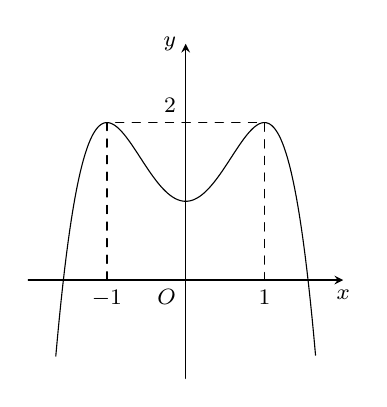
\begin{tikzpicture}[font=\footnotesize, line join=round, line cap=round, >=stealth]
        \draw[->] (-2,0)--(2,0) node[below]{$x$};
        \draw[->] (0,-1.25)--(0,3) node[left]{$y$};
        \draw[dashed] (-1,0)node[below]{$-1$}|-(0,2)node[above left]{$2$}-|(1,0)node[below]{$1$}
        (0,0)node[below left]{$O$};
        \draw[domain=-1.65:1.65,samples=150] plot(\x,{-(\x)^4+2*(\x)^2+1});
    \end{tikzpicture}
}
\end{ex}

\begin{ex}%Câu 2
    Thống kê điểm kiểm tra giữa kỳ 1 môn Toán của 30 học sinh lớp 12C1 của một trường THPT được ghi lại ở bảng sau:\\
    \centerline{\begin{tabular}{|c|c|c|c|c|}
            \hline
            Điểm & $\left[2;4\right)$ & $\left[4;6\right)$ & $\left[6;8\right)$ & $\left[8;10\right)$\\
            \hline
            Số học sinh & $ 4$ & $ 8$ & $ 11$ & $ 7$\\
            \hline
    \end{tabular}}\\
    Trung vị của mẫu số liệu gốc thuộc khoảng nào trong các khoảng dưới đây?
    \choice
    {$\left[2;4\right)$}
    {$\left[4;6\right)$}
    {\True $\left[6;8\right)$}
    {$\left[8;10\right)$}
\end{ex}

\begin{ex}%Câu 3
    Trong không gian $Oxyz$ , một vectơ pháp tuyến của mặt phẳng $\dfrac{x}{-2}+\dfrac{y}{-1}+\dfrac{z}{3}=1$ là
    \choice
    {\True $\overrightarrow{n}=(3;6;-2)$}
    {$\overrightarrow{n}=(2;-1;3)$}
    {$\overrightarrow{n}=(-3;-6;-2)$}
    {$\overrightarrow{n}=(-2;-1;3)$}
\end{ex}

\begin{ex}%Câu 4
    Cho cấp số cộng $\left(u_n\right)$ với số hạng đầu $u_1=-6$ và công sai $d=4$. Tính tổng $S$ của $14$ số hạng đầu tiên của cấp số cộng đó.
    \choice
    {$S=46$}
    {$S=308$}
    {$S=644$}
    {\True $S=280$}
\end{ex}

\begin{ex}%Câu 5
    Cho tứ diện đều $ABCD$ có cạnh bằng $a$. Tích vô hướng $\overrightarrow{AB}\cdot\overrightarrow{AC}$ bằng
    \choice
    {$a^2$}
    {$-a^2$}
    {\True $\dfrac{1}{2}{a^2}$}
    {$\dfrac{\sqrt{3}}{2}{a^2}$}
\end{ex}

\begin{ex}%Câu 6
    Giá trị lớn nhất của hàm số $f(x)=x^3-8x^2+16x-9$ trên đoạn $\left[1;3\right]$ là 
    \choice
    {$\max\limits_{\left[1;3\right]}f(x)=0$}
    {\True $\max\limits_{\left[1;3\right]}f(x)=\dfrac{13}{27}$}
    {$\max\limits_{\left[1;3\right]}f(x)=-6$}
    {$\max\limits_{\left[1;3\right]}f(x)=5$}
\end{ex}

\begin{ex}%Câu 7
    Trong một phép thử với $ A$, $B$ là hai biến cố bất kì, biết rằng $ P(A)=0{,}5$; $ P\left(AB\right)=0{,}3$. Khi đó $ P(B|A)$ bằng
    \choice
    {\True $ 0{,}6$}
    {$ 0{,}15$}
    {$ 0{,}7$}
    {$ 0{,}35$}
\end{ex}

\begin{ex}%Câu 8
    Cho biết $\int\limits_1^3f(x)\mathrm{\,d}x=3$, giá trị của $\int\limits_1^3\dfrac{1}{3}f(x)\mathrm{\,d}x$ bằng
    \choice
    {$ 2$}
    {\True $ 1$}
    {$\dfrac{1}{3}$}
    {$ 3$}
\end{ex}

\begin{ex}%Câu 9
    Tập nghiệm của bất phương trình $2^x\le 4$ là
    \choice
    {\True $\left(-\infty;2\right]$}
    {$\left[0;2\right]$}
    {$\left(-\infty;2\right)$}
    {$\left(0;2\right)$}
\end{ex}

\begin{ex}%Câu 10
    Phát biểu nào sau đây là đúng?
    \choice
    {$\int\dfrac{1}{x}\mathrm{\,d}x=\left| x\right|+C$}
    {\True $\int\dfrac{1}{x}\mathrm{\,d}x=\ln \left| x\right|+C$}
    {$\int\ln x\mathrm{\,d}x=x+C$}
    {$\int\ln\left| x\right|\mathrm{\,d}x=\ln x+C$}
\end{ex}

\begin{ex}%Câu 11
    Bạn An rất thích nhảy hiện đại. Thời gian tập nhảy mỗi ngày của bạn An được thống kê lại ở bảng sau:\\
    \centerline{\begin{tblr}{
                colspec={|c|c|c|c|c|c|},
                hlines,
                vlines,
            }
            Thời gian (phút) & [20;25) & [25;30) & [30;35) & [35;40) & [40;45) \\
            Số ngày & 6 & 6 & 4 & 1 & 1 \\
    \end{tblr}}
    Độ lệch chuẩn của mẫu số liệu ghép nhóm có giá trị gần nhất với giá trị nào dưới đây?
    \choice
    {$ 31{,}25$}
    {$ 31{,}26$}
    {$ 5{,}4$}
    {\True $ 5{,}6$}
\end{ex}

\begin{ex}%Câu 12
    Trong không gian với hệ tọa độ $Oxyz$ , cho đường thẳng $\Delta :\dfrac{x-2}{-3}=\dfrac{y}{1}=\dfrac{z+1}{2}$. Gọi $M$ là giao điểm của $\Delta $ với mặt phẳng $(P):x+2y-3z+2=0$ . Tọa độ điểm $M$ là
    \choice
    {$ M\left(2;0;-1\right)$}
    {$ M\left(5;-1;-3\right)$}
    {$ M\left(1;0;1\right)$}
    {\True $ M\left(-1;1;1\right)$}
        \end{ex}
\Closesolutionfile{ans}
\cauds
\Opensolutionfile{ans}[ans/ans-HXN-\sode-TF]
%Câu hỏi

\begin{ex}%Câu 13
% \immini
% {
    Năm $2025$, báo Giáo dục đã có cuộc khảo sát tại một trường đại học và thấy rằng có $40\%$ sinh viên quan tâm đến chương trình học bổng A; có $17\%$ trong số những sinh viên quan tâm đến học bổng A cũng đã quan tâm đến học bổng B. Qua khảo sát họ cũng thấy rằng có $20\%$ sinh viên quan tâm đến chương trình học bổng B. Người ta chọn ngẫu nhiên một sinh viên từ trường đại học này để thăm dò ý kiến.
% }
% {
%     \includegraphics[width=6cm]{img/HXN-1-13}
% }
    \choiceTF
    {Xác suất để sinh viên được được chọn quan tâm cả hai chương trình học bổng bằng $0{,}062$}
    {Xác suất để sinh viên quan tâm học bổng A nếu biết rằng họ đã quan tâm học bổng B bằng $0{,}4$}
    {Xác suất để sinh viên không quan tâm đến cả chương trình A lẫn học chương trình B bằng $0{,}41$}
    {\True Sinh viên được chọn cho rằng mình có quan tâm đến học bổng $B$; hai hôm sau một nhà báo khác quay lại trường và tiếp tục chọn ngẫu nhiên một sinh viên để thăm dò ý kiến thì gặp được một sinh viên quan tâm đến học bổng $B$, xác suất để người này không quan tâm đến học bổng A bằng $0{,}66$}
   \loigiai{
       Gọi $A$ là biến cố: \lq\lq Sinh viên quan tâm đến học bổng $A$\rq\rq và $B$ là biến cố: \lq\lq Sinh viên quan tâm đến học bổng $B$\rq\rq.\\
       Theo giả thiết ta có $P(A)=0{,}4$; $P\left(B|A\right)=0{,}17$; $P(B)=0{,}2$.\\
       Từ đây ta có sơ đồ hình cây như sau:\\
       \centerline{\includegraphics[width=6cm]{img/HXN-1-13-LG}}
       \begin{itemchoice}
           \itemch 
           Ta có $P(AB)=P(A)\cdot P\left(B|A\right)=0{,}4\cdot 0{,}17=0{,}068$.
           \itemch Ta có $P\left(A|B\right)=\dfrac{P(AB)}{P(B)}=\dfrac{0{,}068}{0{,}2}=0{,}34$.
           \itemch Ta có $P\left(A\cup B\right)=P(A)+P(B)-P(AB)=0{,}4+0{,}2-0{,}068=0{,}532$.\\
           Do đó $P\left(\bar{A}\bar{B}\right)=1-P\left(A\cup B\right)=1-0{,}532=0{,}468$.
           \itemch Ta có $P\left(\bar{A}|B\right)=\dfrac{P\left(\bar{A}B\right)}{P(B)}=\dfrac{P(B)-P(AB)}{P(B)}=\dfrac{0{,}2-0{,}068}{0{,}2}=0{,}66$.\\
           Vì hai cuộc khảo sát là độc lập nên lần chọn đầu không ảnh hưởng đến lần chọn sau, xác suất cần tính là $P\left(\bar{A}|B\right)=0{,}66$.
       \end{itemchoice}
   }
\end{ex}

\begin{ex}%Câu 14
\immini
{
    Cho hàm số $y=\mathrm{e}^x$ có đồ thị $(C)$. Hình phẳng $(\mathscr{D})$ giới hạn bởi các đồ thị $(C)$, tiếp tuyến của $(C)$ tại điểm $ M\left(1;e\right)$ và đường thẳng $ y=-\dfrac{1}{e}x$ được tô đậm như hình vẽ.
    \choiceTF
    {Phương trình tiếp tuyến của $(C)$ tại điểm $ M\left(1;e\right)$ là $y=e\cdot x+e$}
    {\True Đường thẳng $ y=-\dfrac{1}{e}x$ cắt đồ thị $(\mathscr{D})$ tại điểm $\left(-1;\dfrac{1}{e}\right)$}
    {\True Diện tích hình phẳng $(H)$ bằng $0{,}81$ (làm tròn đến hàng phần trăm)}
    {Khi quay hình $(\mathscr{H})$ quanh trục hoành thì được khối tròn xoay có thể tích bằng $3{,}03$ (làm tròn đến hàng phân trăm)}
}
{
   \includegraphics[width=6cm]{img/HXN-1-14}
}
    
    \loigiai{
        \begin{itemchoice}
            \itemch Phương trình tiếp tuyến của $(C)$ tại điểm $M(1;e)$ là $y=y'(1)(x-1)+e$ hay $y=ex$.
            \itemch Toạ độ giao điểm của $(C)$ và đường thẳng $y=-\dfrac{1}{e}x$ thỏa mãn $\heva{& e^x=-\dfrac{1}{e}x \\& y=e^x } \Leftrightarrow \heva{& x=-1 \\& y={e^{-1}}=\dfrac{1}{e}.} $
            \itemch Dễ thấy đường thẳng $y=ex$ cắt đường thẳng $y=-\dfrac{1}{e}x$ tại điểm có hoành độ $x=0$ và cắt đồ thị $(C)$ tại điểm có hoành độ $x=1$.\\
            Do đó diện tích hình phẳng (H) là $S=\int\limits_{-1}^0{\left(\mathrm{e}^x+\dfrac{1}{e}x\right)\mathrm{\,d}x}+\int\limits_0^1{\left(\mathrm{e}^x-ex\right)\mathrm{\,d}x}\approx0{,}81$.
            \itemch Thể tích khối tròn xoay là $V=\pi \int\limits_{-1}^1{\left(e^x\right)^2\mathrm{\,d}x}-\pi \int\limits_{-1}^0{\left(-\dfrac{1}{e}x\right)^2\mathrm{\,d}x}-\pi\int\limits_0^1{(ex)^2\mathrm{\,d}x}\approx 3{,}51$.
        \end{itemchoice}
    }
\end{ex}

\begin{ex}%Câu 15
\immini
{
Hai thành phố cách nhau một con sông. Lấy $A$ và $B$ lần lượt là hai điểm mốc của hai thành phố trong việc đo đạc, đơn vị là km. Người ta xây dựng một cây cầu $EF$ bắc qua sông biết rằng vị trí $A$ cách con sông một khoảng $AH=5$km và vị trí B cách con sông một khoảng là $BK=7$km (xem hình vẽ), biết $HE+KF=24km$ và độ dài $EF$ không đổi.
Đặt $HE=x$ (km), với $x\in\left(0;24\right)$.
}
{
    \includegraphics[width=6cm]{img/HXN-1-15}
}
    \choiceTF
    {\True $AE=\sqrt{25+x^2}$(km), $BF=\sqrt{49+\left(24-x\right)^2}$(km)}
    {Tổng quãng đường đi từ $A$ đến $B$ bằng $\sqrt{25+x^2}+\sqrt{49+x^2}+EF$ (km)}
    {\True Nếu đặt $f(x)=AE+BF$ (km) thì $f'(x)=\dfrac{x}{\sqrt{x^2+25}}+\dfrac{x-24}{\sqrt{x^2-48x+625}}$, $\forall x\in\left(0;24\right)$}
    {Người ta muốn đi từ $A$ đến $B$ theo quãng đường ngắn nhất thì họ phải xây cầu sao cho khoảng cách hai điểm $E$, $H$ bằng $9$ km}
    \loigiai{
        \begin{itemchoice}
            \itemch Với $HE=x$ thì $FK=24-x$ ($0<x<24$).\\
            Ta có $\heva{& AE=\sqrt{25+x^2} \\& BF=\sqrt{49+(24-x)^2}.} $
            \itemch Tổng quãng đường đi từ $A$ đến $B$ là $AE+EF+BF=\sqrt{25+x^2}+\sqrt{49+(24-x)^2}+EF$ (km).
            \itemch Xét hàm số $f(x)=\sqrt{x^2+25}+\sqrt{x^2-48x+625}$;
            $f'(x)=\dfrac{x}{\sqrt{x^2+25}}+\dfrac{x-24}{\sqrt{x^2-48x+625}}$, $\forall x\in (0;24)$.
            \itemch Ta cần tổng quãng đường $AE+EF+FB$ ngắn nhất, mà $EF$ không đổi nên $AE+FB$ bé nhất. \\
            Ta có $f'(x)=\dfrac{x}{\sqrt{x^2+25}}+\dfrac{x-24}{\sqrt{x^2-48x+625}}$, $\forall x\in (0;24)$; $f'(x)=0\Rightarrow x=10$.\\
            Bảng biến thiên \\
            \centerline{
\begin{tikzpicture}[>=stealth]
                    \tkzTabInit[nocadre=false,lgt=1.2,espcl=2.5,deltacl=0.5]{$x$/.7 ,$f'(x)$/.7,$f(x)$/2}
                    {$0$ , $10$ , $24$}
                    \tkzTabLine{ ,-,$0$,+,}
                    \tkzTabVar{+/,-/$12\sqrt{5}$,+/}
                \end{tikzpicture}}
            Ta có $\min\limits_{(0;24)} f(x)=12\sqrt{5}$; khi đó $x=10$km  và $BF=7\sqrt{5}$km $\approx 15{,}65$km.
        \end{itemchoice}
    }
\end{ex}

\begin{ex}%Câu 16
\immini
{
    Trong Dragon Ball, quả cầu Genki là chiêu thức lợi hại mà Son Goku thường sử dụng khi gặp những đối thủ lớn. Được biết trong trận đánh với Frieza đại đế, cuộc chiến có liên quan đến vận mệnh vũ trụ, Goku đã dùng quả cầu này để tung đòn tuyệt sát với Frieza.\\
Chọn hệ trục tọa độ $Oxyz$ thích hợp, đơn vị trên mỗi trục là mét, mặt phẳng $Oxy$ là mặt đất và tia $Oz$ hướng lên trời, Son Goku đứng ở vị trí $ A\left(5;0;40\right)$, Frieza đại đế đứng ở vị trí $ B\left(85;60;40\right)$. Trước khi Goku tạo ra quả cầu Genki thì Frieza đã tấn công phủ đầu, hắn lao về phía Goku với vận tốc $50$ m/s.
}
{
    \includegraphics[width=5cm]{img/HXN-1-16}
}
\choiceTF
    {\True Frieza sẽ mất $2$ giây để đến được vị trí Goku đang đứng}
    {Vectơ vận tốc của Frieza là $\vec{v}=\left(400;300;0\right)$, đơn vị: m/s}
    {\True Sau khi tránh được đòn hiểm từ Frieza, Goku đứng ở vị trí $ C\left(8;-1;46\right)$ đã tạo ra quả cầu Genki được mô hình hóa với phương trình $\left(x-8\right)^2+\left(y+1\right)^2+\left(z-58\right)^2=100$. Khoảng cách bé nhất từ vị trí $ D\left(-182;159;45\right)$ mà Frieza đang đứng đến quả cầu bằng $ 238{,}7$m (kết quả làm tròn đến hàng phần chục)}
    {\True Quả cầu được Goku ném về phía Fide với vận tốc lên đến $ 64$ m/s. Cứ sau mỗi giây thì bán kính nó tăng lên $1$ mét. Nếu Frieza không di chuyển thì sau 3,67 giây (làm tròn đến hàng phần trăm của giây) quả cầu Genki đến được vị trí của Frieza}
    \loigiai{
        \begin{itemchoice}
            \itemch Ta có $\vec{BA}=(-80;-60;0)$ và $AB=\sqrt{(-80)^2+(-60)^2}=100$ m.\\
            Thời gian để Frieza bay từ $B$ đến $A$ để tấn công Goku là $\dfrac{100}{50}=2$s.
            \itemch Vectơ vận tốc của Frieza có dạng $\vec{v}=k\vec{BA}=(-80k;-60k;0)$, với tham số $k>0$.\\
            Ta có $\left| {\vec{v}} \right|=50\Rightarrow \sqrt{(-80k)^2+(-60k)^2}=50\Rightarrow 100|k|=50\Rightarrow k=\dfrac{1}{2}>0$.\\
            Do đó Frieza bay đến chỗ Goku với vectơ vận tốc $\vec{v}=(-40;-30;0)$.
            \itemch Quả cầu Genki có tâm $I(8;-1;58)$, bán kính $R=10\,m$.\\
            $ID=\sqrt{\left(-182-8\right)^2+(159+1)^2+(45-58)^2}=\sqrt{61\,869}\,m\approx 248{,}7\,m$.\\
            Khoảng cách ngắn cần tính là $ID-R=\sqrt{61\,869}-10\approx 238{,}7\,m$.
            \itemch Sau $t$ giây, điểm $M$ (thuộc mặt cầu gần Frieza nhất) di chuyển đoạn đường: $64t+t=65t$ (m).\\
            Khi $M$ chạm vào Frieza (nếu hắn đứng yên) thì $ID-R=65t\Rightarrow t=\dfrac{ID-R}{65}\approx 3{,}67$ (giây).
        \end{itemchoice}
    }
\end{ex}
\Closesolutionfile{ans}
\caukq
\Opensolutionfile{ans}[ans/ans-HXN-\sode-SA]
%Câu hỏi

\begin{ex}%Câu 17
\immini
{
        Một cái ly nước hình hình trụ có chiều cao 9 cm. Lượng nước trong ly chiếm $\dfrac{2}{3}$ thể tích ly nước. Hoa đặt một viên kim cương hình lập phương vào miệng ly nước thì thấy một đỉnh của viên kim cương chạm vào mặt nước, đồng thời mô hình ly nước và kim cương cùng lấy trục ly nước làm trục đối xứng. Nếu ban đầu Hoa đổ nước đầy ly thì sau khi đặt khối lập phương như trên, lượng nước tràn ra là bao nhiêu cm khối (làm tròn đến hàng phần chục và bỏ qua độ dày của ly)?
    \shortans{23,4}
}
{
    \includegraphics[width=3cm]{img/HXN-1-17}
}
\loigiai{
\immini
{
    Xét hình chóp tam giác đều $SABC$ trong đó $S$ là đỉnh của hình lập phương nằm bên trong ly nước và $A$, $B$, $C$ là các điểm chung của kim cương với miệng ly; $O$ là trọng tâm tam giác $ABC$ và $H$ là trung điểm $BC$. \\
Đặt $x$ (cm) là cạnh đáy hình chóp thì\\
\centerline{
    $AO=\dfrac{2}{3}AH=\dfrac{2}{3}\cdot \dfrac{x\sqrt{3}}{2}=\dfrac{x\sqrt{3}}{3}$.
}
Vì hình chóp $S.ABC$ có $SA$, $SB$, $SC$ bằng nhau và đôi một vuông góc (tại $S$) nên $SA=SB=SC=\dfrac{x}{\sqrt{2}}$.\\
Từ đó suy ra $SO=\sqrt{SA^2-OA^2}=\sqrt{\dfrac{x^2}{2}-\dfrac{x^2}{3}}=\dfrac{x\sqrt{6}}{6}$.
}
{
    \includegraphics[width=6cm]{img/HXN-1-17-LG}
}
Theo giả thiết thì chiều cao hình chóp $S.ABC$ bằng $\dfrac{1}{3}$ chiều cao ly nước, tức là $SO=\dfrac{1}{3}\cdot 9=3$.\\
Khi đó $ \dfrac{x\sqrt{6}}{6}=3\Rightarrow x=3\sqrt{6}$ cm.\\
Ta biết rằng thể tích nước tràn ra bằng với thể tích khối chóp $S.ABC$.\\
Thể tích đó là 
$V=\dfrac{1}{3}SO\cdot S_{ABC}=\dfrac{1}{3}\cdot 3\cdot \dfrac{\left(3\sqrt{6}\right)^2\sqrt{3}}{4}=\dfrac{27\sqrt{3}}{2}\approx 23{,}4$ cm$^3$.
}
    \end{ex}
    
    \begin{ex}%Câu 18
% \immini
% {
    Một người công nhân có thể sản xuất với tốc độ là\\
    $q(t)=100+\mathrm{e}^{-0{,}5t}$ đơn vị sản phẩm trong $1$ giờ, với $t$ (giờ) là thời gian tính từ khi bắt đầu làm việc. Biết rằng người công nhân bắt đầu làm việc từ lúc $8$ giờ sáng, hỏi người đó sẽ sản xuất được bao nhiêu đơn vị sản phẩm trong khoảng thời gian từ $9$ giờ sáng đến $11$ giờ trưa (làm tròn đến hàng đơn vị)?
\shortans{201}
% }
% {
%     \includegraphics[width=6cm]{img/HXN-1-18}
% }
\loigiai{
Gọi $Q(t)$ là số đơn vị sản phẩm mà công nhân sản xuất được sau $t$ giờ tính từ lúc $8$ giờ sáng.\\
Ta có $Q'(t)=q(t)=100+{\mathrm{e}^{-0{,}5t}}$.
Số đơn vị sản phẩm người đó sản xuất được từ $9$ giờ sáng ($t=1$) đến $11$ giờ trưa ($t=3$) là\\
$Q(3)-Q(1)=\int\limits_1^3{q(t)\mathrm{\,d}t}=\int\limits_1^3\left(100+{e^{-0.5t}}\right)\mathrm{\,d}t \approx 201$ (đơn vị sản phẩm).
}
\end{ex}

\begin{ex}%Câu 19
\immini
{
    Mảnh đất vườn của nhà anh Điệp có một phần ranh giới cũng là một phần đường cong $(C)\colon y=\dfrac{x+a}{x+b}$, bao quanh nó là sông nước. Với hệ trục tọa độ $Oxy$ thích hợp, đơn vị trên mỗi trục là $10$ mét thì đường cong $(C)$ đi qua điểm $\left(2;3\right)$ và có đường tiệm cận đứng $x=1$. Hàng ngày anh Điệp phải dùng thuyền máy để vận chuyển trái cây từ khu vườn của mình đến hai tuyến đường $\Delta_1\colon 2x+y-4=0$ và $\Delta_2\colon x+2y-2=0$ cho những người lái buôn từ nơi khác đến.
}
{
    \includegraphics[width=6cm]{img/HXN-1-19}
}
Anh Điệp cần xác định một vị trí $ M\left(x_0;y_0\right)$ thuộc khu vườn của mình để tổng các khoảng cách từ vị trí M đó đến hai tuyến đường $\Delta_1,\Delta_2$ là bé nhất. Hỏi khoảng cách từ vị trí được chọn làm gốc tọa độ đến điểm M là bao nhiêu mét (làm tròn đến hàng phần chục)?
\shortans{34,1}
\loigiai{
Đồ thị hàm số có tiệm cận đứng $x=-b=1\Rightarrow b=-1$.\\
Khi đó đồ thị hàm số $y=\dfrac{x+a}{x-1}$ qua $(2;3)\Rightarrow 3=\dfrac{2+a}{2-1}\Rightarrow a=1$; hàm số là $y=\dfrac{x+1}{x-1}$ $(C)$.\\
Gọi $M\left(x_0;\dfrac{x_0+1}{x_0-1}\right)\in (C)$, $x_0>1$. Tổng khoảng cách từ $M$ đến hai đường thẳng $\triangle _1,\triangle _2$ là
\begin{eqnarray*}
    &&d=d\left(M,\triangle_1\right)+d\left(M,\triangle _2\right)=\dfrac{\left| 2x_0+\dfrac{x_0+1}{x_0-1}-4 \right|}{\sqrt{5}}+\dfrac{\left| x_0+2\cdot \dfrac{x_0+1}{x_0-1}-2 \right|}{\sqrt{5}}\\
    &\Leftrightarrow&\sqrt{5}d=\left| \dfrac{2x_0^2-5x_0+5}{x_0-1} \right|+\left| \dfrac{x_0^2-x_0+4}{x_0-1} \right|=\dfrac{2x_0^2-5x_0+5}{x_0-1}+\dfrac{x_0^2-x_0+4}{x_0-1}\\
    &&\left(\text{vì } \heva{& 2x_0^2-5x_0+5>0 \\& x_0-1>0 \\& x_0^2-x_0+4>0 },\,\forall x_0>1\right)
\end{eqnarray*}
Đặt $\sqrt{5}d=\dfrac{3x_0^2-6x_0+9}{x_0-1}=g(x)$ với $x>1$.\\
Ta có: $g'(x)=\dfrac{3x_0^2-6x_0-3}{\left(x_0-1\right)^2}$; $g'(x)=0\Rightarrow 3x_0^2-6x_0-3=0\Rightarrow x_0=1+\sqrt{2}>1$.\\
Ta có $\min \limits_{\left(1;+\infty \right)}\,g(x)=g\left(1+\sqrt{2}\right)=6\sqrt{2}\Rightarrow \sqrt{5}d\ge 6\sqrt{2}\Rightarrow d\ge \dfrac{6\sqrt{10}}{5}$.\\
Dấu đẳng thức xảy ra khi $x_0=1+\sqrt{2} \Rightarrow M\left(1+\sqrt{2};1+\sqrt{2}\right)$.\\
Khoảng cách OM trên thực tế là $10\times \sqrt{\left(1+\sqrt{2}\right)^2+\left(1+\sqrt{2}\right)^2}=10\times \left(1+\sqrt{2}\right)\sqrt{2}\approx 34{,}1$ mét.
}
\end{ex}

\begin{ex}%Câu 20
\immini
{
    Một tên trộm đang cố gắng kéo thùng nữ trang qua một bức tường có độ dày $ BC=1m$; biết rằng tường cao $4$ m và sợi dây được kéo theo đường gấp khúc $ABCD$ có độ dài không đổi bằng $20$ m, đoạn $ BF=0{,}5m$. Trong khi kéo thì tên trộm luôn ghì đầu dây theo một thanh vịn của cầu thang (đầu dây dịch chuyển theo phương $AF$). Biết rằng thanh vịn cầu thang hợp với phương ngang một góc bằng $30^{\circ}$.
}
{
    \includegraphics[width=10cm]{img/HXN-1-20}
}
Khi hai chú cảnh sát xuất hiện thì vị trí $A$ cách F khoảng $6$ m và thùng $D$ tiến về phía $E$ với tốc độ $1$ m/s. Hỏi đầu dây $A$ rời xa điểm $F$ với tốc độ bao nhiêu m/s? (Làm tròn kết quả đến hàng phần trăm).
\shortans{0,95}
\loigiai{
Đặt $DE=x$(m), $AF=y$(m).\\
Ta có $CD=\sqrt{x^2+16}$ và $\widehat{AFB}=180^{\circ }-60^{\circ }=120^{\circ }$.\\
Suy ra $AB=\sqrt{y^2+0{,}5^2-2.0{,}5\cdot y\cos 120^{\circ }}=\sqrt{y^2+0{,}5y+0{,}25}$.\\
Ta có $AB+CD+1=20\Leftrightarrow \sqrt{x^2+16}+\sqrt{y^2+0{,}5y+0{,}25}=19$ \tagEX{*}
Thay $y=6$ vào $(*)$ ta được $\sqrt{x^2+16}+\sqrt{6^2+0{,}5.6+0{,}25}=19\Rightarrow x\approx 12{,}1$  (Lưu vào A).\\
Đạo hàm hai vế của $(*)$ theo biến $t$ ta được:\\
$\dfrac{x}{\sqrt{x^2+16}}\cdot \dfrac{\mathrm{\,d}x}{\mathrm{\,d}t}+\dfrac{2y+0{,}5}{2\sqrt{y^2+0{,}5y+0{,}25}}\cdot \dfrac{dy}{\mathrm{\,d}t}=0$ \tagEX{**}
Thay $y=6$ m; $x=A\approx 12{,}1$ m; $\dfrac{\mathrm{\,d}x}{\mathrm{\,d}t}=-1$ m/s (do $x$ ngày càng giảm theo thời gian $t$) vào $(**)$ ta tính được $\dfrac{dy}{\mathrm{\,d}t}\approx 0{,}95$ m/s hay đầu dây $A$ rời xa điểm $F$ với tốc độ khoảng $0{,}95$ m/s.
}
\end{ex}

\begin{ex}%Câu 21
\immini
{
Trong công trường xây dựng, có một bộ khung sắt hình lập phương như hình vẽ (ta xem nó là hình lập phương dạng $ 2\times 2\times 2$). Người ta nhìn thấy một con kiến và một con gián xuất phát cùng lúc trên hai đỉnh thuộc đường chéo lớn của khung sắt hình lập phương và di chuyển trên các cạnh của mỗi hình vuông nhỏ. Con kiến cần đến vị trí mà con gián xuất phát và ngược lại, mỗi con ngày càng di chuyển xa vị trí mà nó xuất phát. Tính xác suất để hai con côn trùng này gặp nhau biết rằng vận tốc của gián bằng 4 cm/s, vận tốc của kiến là 2 cm/s. Kết quả được làm tròn đến hàng phần trăm.
\shortans{0,27}
}
{
    \includegraphics[width=6cm]{img/HXN-1-21}
}
\loigiai{
\immini
{
    Ta xem mỗi bước di chuyển của mỗi con là 1 đơn vị (ứng với cạnh hình vuông nhỏ).\\
Để đi hết hành trình của mình thì gián cần đi xuống $2$ đơn vị, sang trái $2$ đơn vị và đi dọc $2$ đơn vị (có tất cả là 6 bước di chuyển) nên số cách đi của gián là $\mathrm{C}_6^2\mathrm{C}_4^2$; hoàn toàn tương tự kiến cũng có số cách đi là $\mathrm{C}_6^2\mathrm{C}_4^2$.\\
Gọi $\Omega $ là không gian mẫu thì $n\left(\Omega \right)=\left(C_6^2C_4^2\right)^2$.\\
Vận tốc của gián gấp đôi vận tốc của kiến nên nếu hai con gặp nhau thì tại vị trí chúng gặp gián đã di chuyển $4$ bước, kiến di chuyển 2 bước. Vị trí hai con gặp nhau (nếu có) được đánh dấu ở $6$ vị trí trên hình vẽ.
}
{
    \includegraphics[width=6cm]{img/HXN-1-21-LG}
}
\begin{itemize}
    \item Tại vị trí $A$: Gián có $2$ lần di chuyển sang trái, $2$ lần di chuyển dọc; sau đó đi từ $A$ đến đích thì nó cần $2$ lần đi xuống. Số cách đi của gián là $\mathrm{C}_4^2\mathrm{C}_2^2\mathrm{C}_2^2$.  Hành trình của kiến cũng tương tự mà theo chiều ngược lại nên kiến có $\mathrm{C}_4^2\mathrm{C}_2^2\mathrm{C}_2^2$ cách đi. Số cách đi hai con là $\left(C_4^2C_2^2C_2^2\right)^2$.\\
    Tại các vị trí $A$, $C$, $E$ thì số cách đi mỗi con là như nhau. 
    \item Tại vị trí $B$: Số cách đi của hai con là  $\left(\mathrm{C}_4^1\mathrm{C}_3^1\mathrm{C}_2^2\mathrm{C}_2^1\right)^2$.\\
    Tại các vị trí $B$, $D$, $F$ thì số cách đi mỗi con là như nhau. 
\end{itemize}
Gọi $X$ là biến cố hai con côn trùng gặp nhau trên đường đi, ta có\\ $P(X)=\dfrac{3\left(\mathrm{C}_4^2\mathrm{C}_2^2\mathrm{C}_2^2\right)^2+3\left(\mathrm{C}_4^1\mathrm{C}_3^1\mathrm{C}_2^2\mathrm{C}_2^1\right)^2}{\left(\mathrm{C}_6^2\mathrm{C}_4^2\right)^2}=\dfrac{17}{75}\approx0{,}27$.
}
\end{ex}

\begin{ex}%Câu 22
Trong không gian $Oxyz$, cho mặt cầu $\left(S_1\right)$ có tâm $ I\left(2;1;1\right)$, bán kính bằng $ 4$ và mặt cầu $\left(S_2\right)$ có tâm $J\left(2;1;5\right)$, bán kính bằng $ 2$. Gọi $(P)$ là mặt phẳng thay đổi tiếp xúc với hai mặt cầu $\left(S_1\right),\left(S_2\right)$ và đặt $T_1,T_2$ lần lượt là giá trị nhỏ nhất, giá trị lớn nhất của khoảng cách từ điểm $ O$ đến $(P)$. Tìm giá trị $ T_1^2+T_2^2$.
\shortans{48}
\loigiai{
\immini
{
    Ta có $IJ=4<R_1+R_2$ (với $R_1=4$, $R_2=2$)  nên hai mặt cầu $\left(S_1\right)$ và $\left(S_2\right)$ cắt nhau.\\
Gọi $M$ là giao điểm của $IJ$ và $(P)$.\\
Ta có $\dfrac{MJ}{MI}=\dfrac{R_2}{R_1}=\dfrac{1}{2}\Rightarrow J$ là trung điểm của $MI$.\\
Suy ra $M(2;1;9)$.
}
{
\includegraphics[width=6cm]{img/HXN-1-22-LG}
}
Gọi $\vec{n}=(a;b;c)$ là vectơ pháp tuyến của $(P)$ với $a^2+b^2+c^2>0$.\\
Phương trình $(P)\colon a(x-2)+b(y-1)+c(z-9)=0$ hay $ax+by+cz-2a-b-9c=0$.\\
Ta có $(P)$ tiếp xúc $\left(S_1\right) \Leftrightarrow d\left(I,(P)\right)=4\Leftrightarrow \dfrac{|8c|}{\sqrt{a^2+b^2+c^2}}=4\Leftrightarrow \dfrac{|2c|}{\sqrt{a^2+b^2+c^2}}=1$.\\
Dễ thấy $c\ne 0$ nên ta có thể chọn $c=1\Rightarrow a^2+b^2=3$.\\
Khi đó $d\left(O,(P)\right)=\dfrac{\left| -2a-b-9c \right|}{\sqrt{a^2+b^2+c^2}}=\dfrac{|2a+b+9|}{2}$\tagEX{1}
Theo bất đẳng thức Cauchy Schwarz thì $|2a+b|\le \sqrt{\left(2^2+1^2\right)\left(a^2+b^2\right)}=\sqrt{5.3}=\sqrt{15}$.\\
Dấu đẳng thức xảy ra khi và chỉ khi $\dfrac{a}{2}=\dfrac{b}{1}$.\\
Do đó 
\begin{align}
    &-\sqrt{15}\le 2a+b\le \sqrt{15} \notag\\
    \Rightarrow& \underbrace{9-\sqrt{15}}_{+}\le 2a+b+9\le 9+\sqrt{15}\notag\\
    \Rightarrow& \underbrace{9-\sqrt{15}}_{+}\le |2a+b+9|\le 9+\sqrt{15} \tag{2}
\end{align}
Từ $(1)$ và $(2)$ suy ra $\dfrac{9-\sqrt{15}}{2}\le d\left(O,(P)\right)=\dfrac{|2a+b+9|}{2}\le \dfrac{9+\sqrt{15}}{2}$.\\
Do đó $T_1=\dfrac{9-\sqrt{15}}{2}$; $T_2=\dfrac{9+\sqrt{15}}{2}$ và $T_1^2+T_2^2=48$.
}
\end{ex}
\Closesolutionfile{ans}
\inputansbox{6,4,3}{ans/ans-HXN-\sode-T,ans/ans-HXN-\sode-TF,ans/ans-HXN-\sode-SA}